\section{Sprint 1}

\subsection{Sprint Planning}
	In this sprint the group were planning on a small delivery. This is because we need a lot of time to get started with the development and get to know the framework Backbone. The delivery in this sprint delivery will include a graphical map with zooming functionality. To get started on implementing the other functional requirements, it requires that we have the map to put them on. 
	In order to start with the other parts of the game, it require that the group have defined and implemented all the elements in the game like building, power plants, power lines, etc.

	To be able to keep up the testing activity in the upcoming sprints, we will try to get started with unit tests. This will probably take some time since testing is a new concept to many in the group as well as Jasmine is a new framework for all in the group. 

\subsubsection{Duration and worklaod}
	When the group had the firs meeting, we agreed to have sprints lasting for 2 weeks.
	After the 10days into the first sprint, the group realised that goal was not reachable.
	The group decided to change the first sprint duration to 3 weeks instead of 2 weeks. \\
	{\bf Duration:} 09.09 - 29.09 \\
	{\bf Workload:} This is the list with hours spent (the whole grup) on the project in this sprint.
	\begin{itemize}
		\item {\bf Planning:} 11 hours
		\item {\bf Development:} 94,5 hours
		\item {\bf Design:} 15 hours
		\item {\bf Documentation (report):} 40,5 hours
	\end{itemize}
	{\bf Total workload: } 161 hours \\
	The group's goal was to work at least 20-25 hours pr/person every week. We did not manage this at this sprint, but we had a avrage of 13,5 hours/week (161 hours/4 persons/3 weeks = 13.5 hours). 
	In section 'problems during the sprint', we have written what have happend during this sprint.
	Many of the scenarios from that section affected the workload on the group. 

\subsubsection{Expected results}


\subsubsection{Sprint backlog}
\begin{tabular}{| p{1cm} | p{8cm} | p{3cm} |}
	\hline
	ID & Description & Estimate \\ \hline
	FR6.1 & The user should be able to see a small part of the game map. & commment \\ \hline
	FR6.2 & The user should be able to navigate around the map using the touch function on the phone & commment \\ \hline
	FR6.4 & The user should be able to view all of the map by double tapping the screen; double tapping a point on the complete map should zoom in on that area. & commment \\
	\hline
\end{tabular}

\subsection{Implementation}

\subsubsection{Models}
We have been using Backbone to implement the game models in this project. In Sprint 1 we have implemented 
the following models to store game data.
\subsubsection*{Building}
The building model stores information about the buildings location on the game map as well as a reference 
to the image that should be drawn on the map.
\subsubsection*{Level}
This model contains the map and player object. It is this object's job to handle the logic responsible for 
updating the state of the game models.
\subsubsection*{Map}
The map model has two main functions. The first is to hold a Backbone Collection with all the buildings 
that are placed on the map. The second is to maintain which part of the map that should be painted.
\subsubsection*{Player} 
The player model stores how many lives the player has and how much money the player has available to them.

\subsubsection{Presenters}
Backbone Presenters are the JavaScript objects that connects the Backbone Models to the visual HTML code. 
They listen to changes to the Backbone Models and changes the HTML objects accordingly. The Presenters also 
handles input events from the HTML objects.
\subsubsection*{Menu Screen}

\subsubsection*{Game Screen}
\subsubsection*{Instruction screen}
\subsubsection*{Highscore screen}

\begin{figure}[!ht]
\centering
\subfigure{
	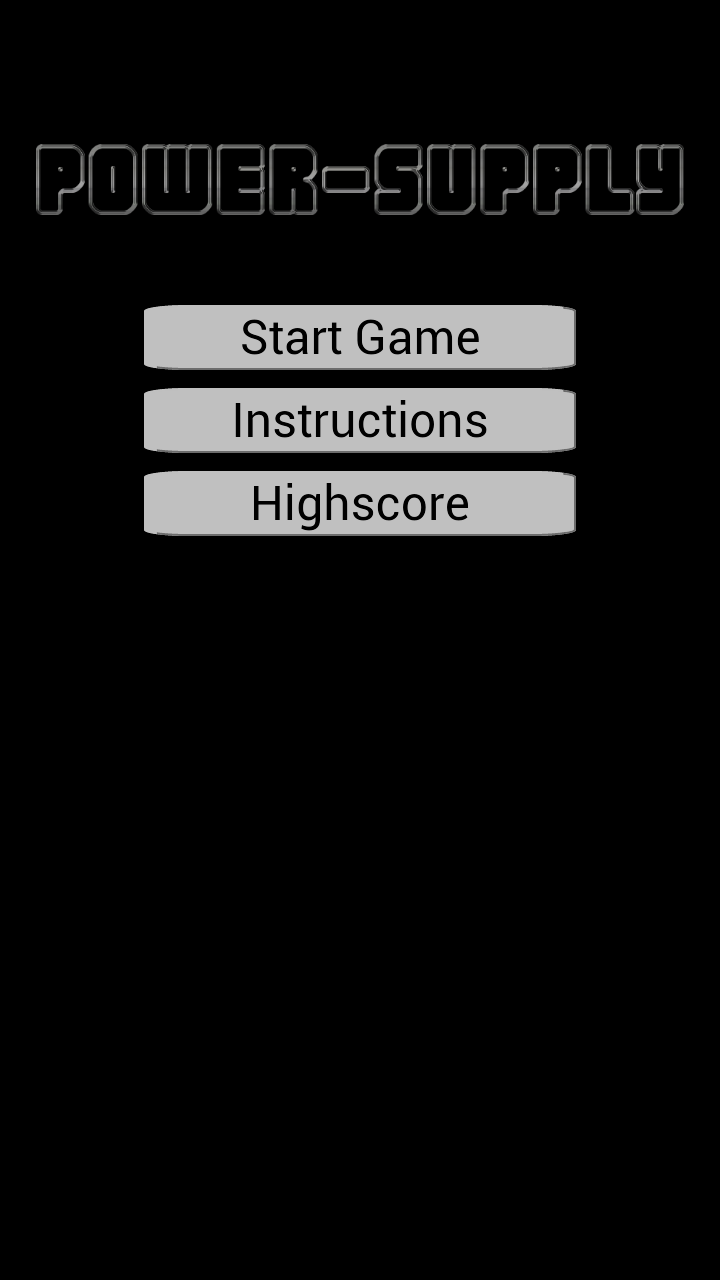
\includegraphics[scale=0.2]{pictures/game_screenshot_2}
}
\subfigure{
	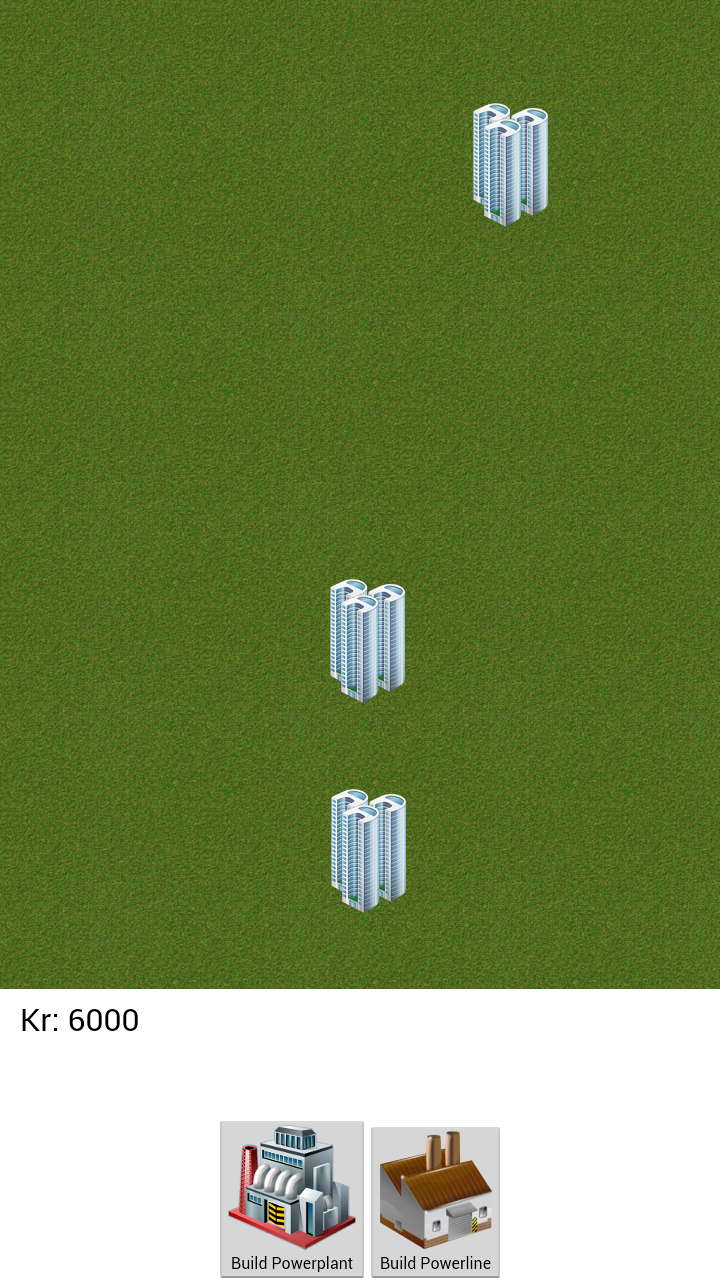
\includegraphics[scale=0.2]{pictures/game_screenshot_1}
}
\end{figure}

\subsubsection{Game Logic}
\subsubsection*{Place buildings on map}

\subsubsection{Other Implementations}
\subsubsection*{Rendering}
\subsubsection*{Game Loop}

\subsection{Testing}

There has been minimal testing in the first sprint. Much time has been spent getting to know the programming tools to be used and the focus has been on creating a base for further programming as well as something more visual to show the customer, as opposed to planning tests to be executed. The testing that has been carried out has been manual testing as well as debugging using Android Debug Monitor. The manual testing has been carried out in parallell with programming using an actual Android phone as well as Android Virtual Device. Android Virtual Device is an emulator configuration that lets one model an actual device by defining hardware and software options to be emulated. This approach has been sufficient for the first sprint, but as the amount of code grows and more logic is added there will be need for more proper testing, such as unit-, integration- and usability testing. More planned out tests will take place in the next and following sprints.

\subsection{Problems during the sprint:}
In the start of this sprint we had a major problem that many of the group members was ill or 
that many members didn't have the time to contribute to the project. This is one of the risk factors 
that we have listed in the risk analysis. 
Apart form that, we had some problems with the group dynamics. The members in the group are 
quite different and like to work in different ways. The main problem was that many of the group members
have different experiences with this kind of group work, technology as well as we have 
different personalities.
We managed to solve this problem by sitting down and discussing the problem. We discovered that
one of the main problems was that the role allocation and the responsability had not been present.
After we allocated the roles with a specific responsability, many of our problems was solved and
we have been able to work better as a group.

Sprint 1 was the first phase in the project with implementation and coding. In the start, many in the group had
some problems with setting up the development environment (specially on windows). We managed
to solve this problem, but it affected the total implementation because the whole group couldn't 
contribute as much as we hopeded. One solution was to go over from windows to ubuntu. 
In the end of the sprint, everyone had a working development environment.

Since no members in the group have alot experience with the technology, it was sometimes hard
to be able to do the implementations fast enough, or even know where to start. 
Hopefully we will not have as much problems in the next sprints, but it is still a risk factor 
since we are still quite inexperienced with javascript, mobile development and the framworks we use. 

\subsection{Customer feedback}
	This is the feeback from the customers and the feedback from us to the customers (good/bad/what could be better?)

\subsection{Sprint retrospective}
	After every sprint we will talk about what we can do better, what to keep and what new to indtroduce to the working process.